%% Full length research paper template
%% Created by Simon Hengchen and Nilo Pedrazzini for the Journal of Open Humanities Data (https://openhumanitiesdata.metajnl.com)

\documentclass{article}
\usepackage[italian]{babel}
\usepackage[utf8]{inputenc}
\usepackage{johd}
\usepackage{graphicx}
\usepackage{graphics}
\usepackage{listings}
\usepackage{color}
    \definecolor{listinggray}{gray}{0.9}
\definecolor{lbcolor}{rgb}{1,1,1}
\lstset{
backgroundcolor=\color{lbcolor},
    tabsize=4,    
%   rulecolor=,
    language=[GNU]C++,
        basicstyle=\scriptsize,
        upquote=true,
        aboveskip={1.5\baselineskip},
        columns=fixed,
        showstringspaces=false,
        extendedchars=false,
        breaklines=true,
        prebreak = \raisebox{0ex}[0ex][0ex]{\ensuremath{\hookleftarrow}},
        frame=single,
        numbers=left,
        showtabs=false,
        showspaces=false,
        showstringspaces=false,
        identifierstyle=\ttfamily,
        keywordstyle=\color[rgb]{0,0,1},
        commentstyle=\color[rgb]{0.026,0.112,0.095},
        stringstyle=\color[rgb]{0.627,0.126,0.941},
        numberstyle=\color[rgb]{0.205, 0.142, 0.73},
%        \lstdefinestyle{C++}{language=C++,style=numbers}’.
}
\lstset{
    backgroundcolor=\color{lbcolor},
    tabsize=4,
  language=C++,
  captionpos=b,
  tabsize=3,
  frame=lines,
  numbers=left,
  numberstyle=\tiny,
  numbersep=5pt,
  breaklines=true,
  showstringspaces=false,
  basicstyle=\footnotesize,
%  identifierstyle=\color{magenta},
  keywordstyle=\color[rgb]{0,0,1},
  commentstyle=\color{green},
  stringstyle=\color{red}
  }


\title{Multipanner - Creazione di un panner per coppie spaziate}

\author{Gabriele Acquafredda$^{a}$$^{*}$ \\
    \small $^{a}$2° Anno di Tecnica Del Suono, Primo livello, Dipartimento di Musica Elettronica\\
    \small  Conservatorio di Musica Niccolò Piccinni, Bari, Italia\\
}

\date{Febbraio 2023} 

\begin{document}

\maketitle

\begin{abstract} 
    \noindent La presente documentazione riguarda la risoluzione di una problematica riscontrata durante una sessione di registrazione in cui v'è stata una coppia spaziata ORTF come main: esiste un modo per mappare lo spazio precisamente mettendolo in relazione con un main ORTF senza la necessità di agire nella post-produzione con degli artefatti e delle approssimazioni? La risposta è stata la costruzione di un panner che ragiona in coordinate spaziali e mette in stretta correlazione ogni spot messo nello spazio con la coppia main, servendoci di poche regole matematiche, in particolar modo trigonometriche e della piattaforma di sviluppo FAUST.
\end{abstract}

\section{La problematica - Perché adoperare il Multipanner}
Stiamo registrando un'orchestra e abbiamo 10 microfoni che mappano lo spazio per sezioni. Abbiamo un microfono per le viole, uno per i contrabbassi ecc. Come coppia main adoperiamo un ORTF che ci riprende sia l'orchestra nella sua interezza che, logicamente, l'ambiente circostante.
Una volta terminato il lavoro di registrazione, importiamo tutte le registrazioni sulla nostra DAW per cominciare a lavorarci. Tutti gli spot che abbiamo adoperato per le sezioni sono logicamente mono, quindi abbiamo la necessità di sincronizzarli con il main per poi posizionarli nell'immagine stereo.
Il panner tradizionale delle DAW, però, non consente né di applicare dei ritardi (se non aggiungendo degli appositi plugin), né di applicare dei ritardi tra i canali di SX e DX - cosa che, nel modello fisico dell'ORTF è naturale: se una sorgente proviene da SX, il canale di DX sarà leggermente sfasato rispetto al canale di SX, ove logicamente la sorgente "arriverà" prima. 
Inoltre il panner tradizionale delle DAW non ragiona con le figure polari del nostro ORTF. Ciò vuol dire che il fatto di stare a n gradi a SX o DX non influenzerà direttamente la resa sonora del nostro panning.
Il panner tradizionale, insomma, ragiona solo in termini di ampiezza di L e di R, non dandoci una vera e propria informazione stereofonica, ma solo un'approssimazione di questa. Un vero panner per mappare lo spazio deve, conseguentemente, non solo ragionare in termini di ampiezza, ma anche in termini di tempo e di fase, in modo da simulare matematicamente (quindi non fisicamente) in tutto e per tutto il comportamento di una sorgente sonora posizionata nello spazio in correlazione ad un dato punto di riferimento. Il punto di riferimento, nel nostro caso, diventa il centro della nostra coppia spaziata, sia questa ORTF, NOS, AB ecc.

\section{Concettualizzazione}

    \subsection{Le 3 dimensioni}
    Il panner tradizionale delle DAW ragiona sulla differenza di ampiezza tra L e R. Nel nostro caso, abbiamo la necessità di costruire una mappa che sia tridimensionale per poi applicarla su ciascuno SPOT. Preso, quindi, come riferimento il punto $\left[0,0,0\right]$, nonché il centro della nostra coppia spaziata e preso un punto dello spazio che identifica il nostro microfono spot $\left[x_a,y_a,\Delta z_a\right]$, dobbiamo permettere al nostro programma di Faust di calcolare in autonomia la distanza effettiva tra $\left[0,0,0\right]$ e $\left[x_a,y_a,\Delta z_a\right]$ e l'angolo di incidenza azimutale. Per questa operazione, disponiamo un semplice disegno tecnico che descrive la situazione:

    \begin{figure}[H]
        \centering
        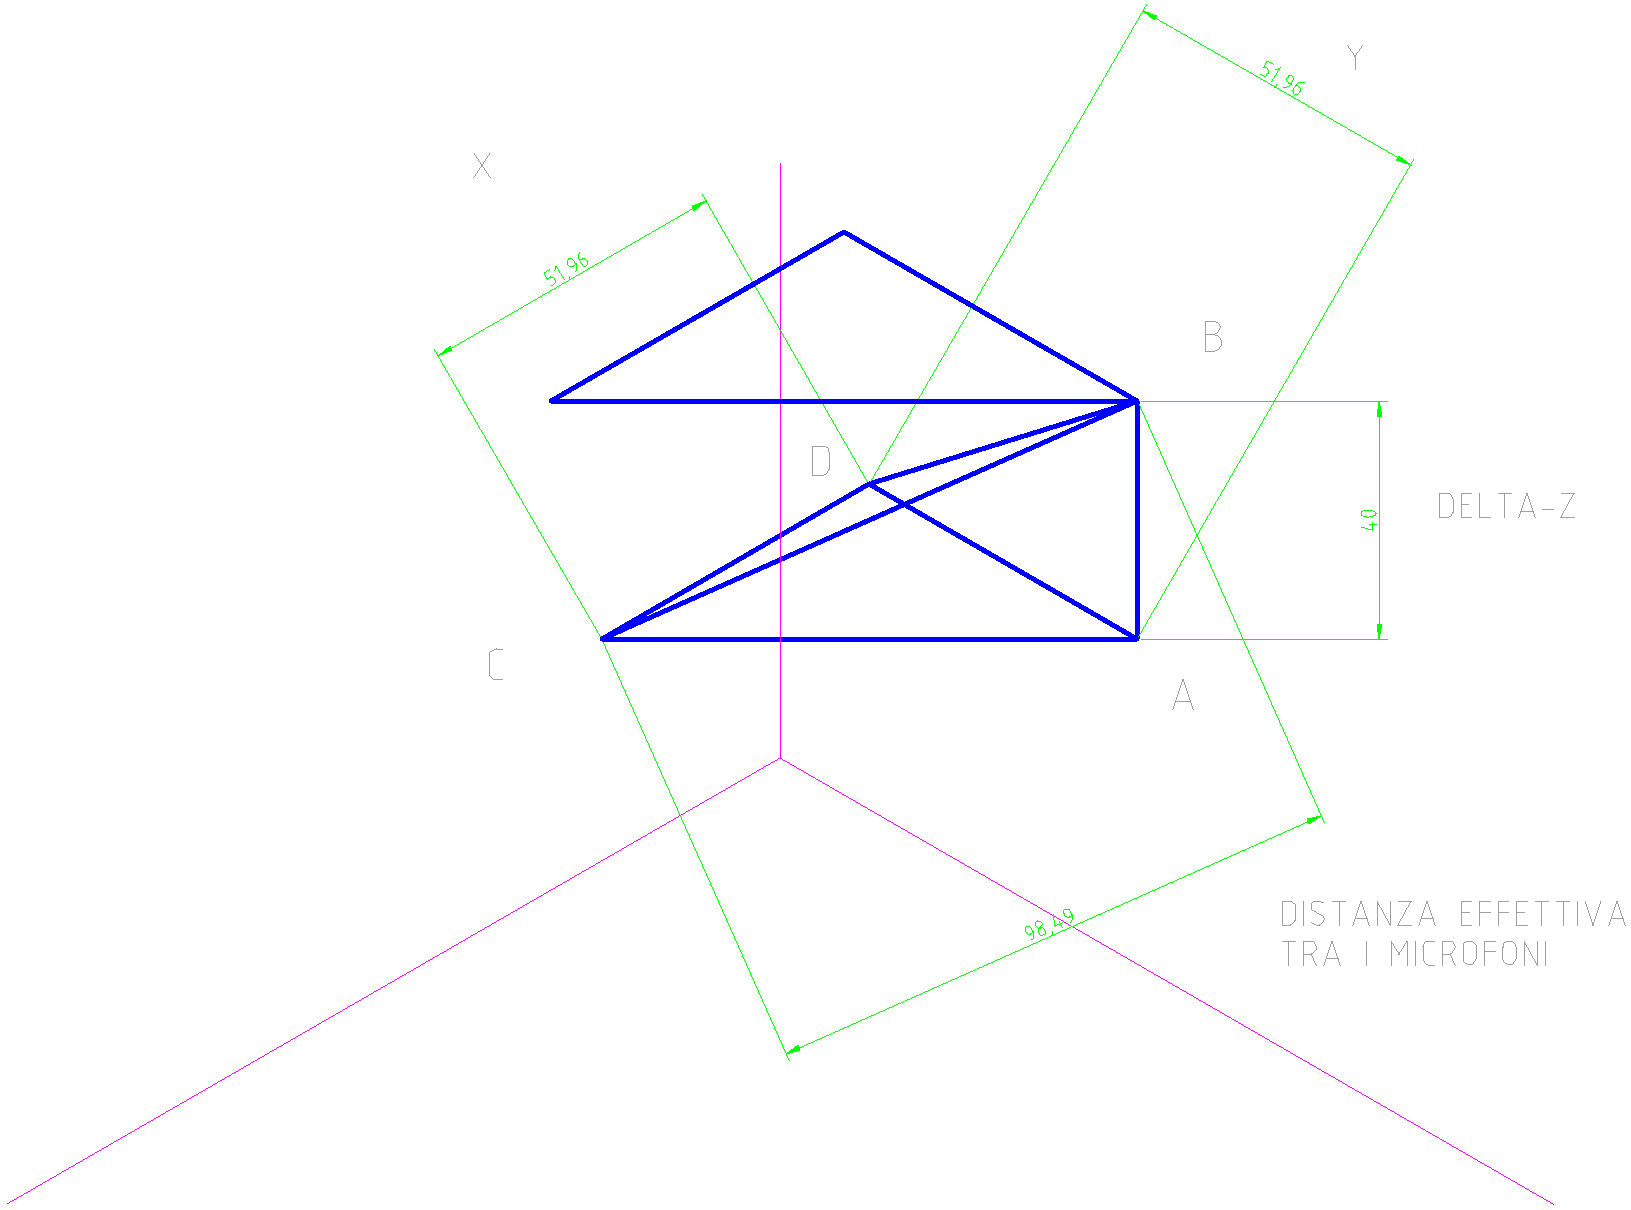
\includegraphics[width=0.7\textwidth]{images/Assonometria.png}
         \caption{\label{fig1}Assonometria}
    \end{figure}

    Per capire meglio la problematica, quindi, costruiamo una piramide a base di triangolare, dove gli estremi contrassegnati con le lettere $B$ e $C$ rappresentano rispettivamente il centro della coppia spaziata e la posizione dello spot. Così facendo, nel nostro programma diamo in input le tre dimensioni $x, y, \Delta z$ che in termini geometrici saranno tradotte in
    $$x = CD$$
    $$y = DA$$
    $$z = AB$$
    Riusciamo quindi a calcolarci la distanza $CB$ attraverso l'applicazione del teorema di Pitagora.
    $$CB = \sqrt{AB^2 + CA ^ 2}$$
    Per conoscere invece l'angolo di incidenza azimutale, ci serviamo dell'applicazione del teorema di Pitagora e del teorema del coseno
    $$BD = \sqrt{AD^2 + BA ^ 2}$$
    $$\widehat{CBD} = arccos \biggl( {CB ^ 2 + BD ^ 2 - CD ^ 2\over 2 * CB * BD} \biggr)$$

    Siccome il teorema di pitagora e il teorema del coseno sono ricorrenti nella formalizzazione del panner, costruiamo delle funzioni matematiche da richiamare dalla nostra libreria di Faust "11ts.lib". In questa libreria verranno comprese anche altre funzioni matematiche ricorrenti.
    
    \begin{lstlisting}
import("stdfaust.lib");
ts = library("12ts.lib");

//conversione da gradi a radianti e viceversa
deg2rad = * (ma.PI/180);
rad2deg = * (180/ma.PI);

//teorema di pitagora
pit(a,b) = sqrt(a ^ 2 + b ^ 2) : float;

//teorema di carnot per il calcolo dell'angolo compreso tra due lati. l1 e l2 sono i lati in cui è compreso l'angolo da calcolare, l3 è il lato opposto
acarnot(l1,l2,l3) = acos((l1 ^ 2 + l2 ^ 2 - l3 ^ 2)/(2 * l1 * l2)) : float;

//teorema di carnot per il calcolo del lato opposto ad un angolo già dato e i due contigui. l1 e l2 sono i lati, rad è l'angolo opposto
lcarnot(l1,l2,rad) = sqrt((l1^2) + ((l2^2) - 2*(l1) * (l2) * cos(rad))) : float;

//simulatore figura polare
ppattern(x,pp,inc,dvg) = x <: ((1-pp) * _) + (pp * _ * cos(inc))*cos(dvg);
    \end{lstlisting}
    
    
    In tale maniera costruiamo un codice pulito e riutilizzabile per qualsiasi nostro progetto.
    Difatti nel nostro progetto di Faust avremo la seguente situazione:
    
    \begin{lstlisting}
//OUTPUT DISTANZA REALE TRA I MICROFONI SULLE TRE COORDINATE
xyz2dst(cd,da,ab) = cb(ab,ca)
with{
    ca = ts.pit(cd,da);
    cb(ab,ca) = ts.pit(ab,ca);
};

//OUTPUT RADIANTI AZIMUT REALI
dst2arad(cd,da,ab) = arad(cb,db,cd,xsign)
with{
    cb = xyz2dst(cd,da,ab);

    xsign = cd : ma.signum;
    db = ts.pit(ab,da);
    arad(cb,db,cd,xsign) = ts.acarnot(cb,db,cd) : ts.rad2deg : _ * xsign : (_+90) : ts.deg2rad;
};
    \end{lstlisting}

    \subsection{La coppia main}
    
    Finora il main è stato considerato come un unico microfono, però, come ben chiaro, il progetto è finalizzato ad avere come main una coppia spaziata. Per comodità consideriamo ora la planimetria del progetto.

    \begin{figure}[H]
        \centering
        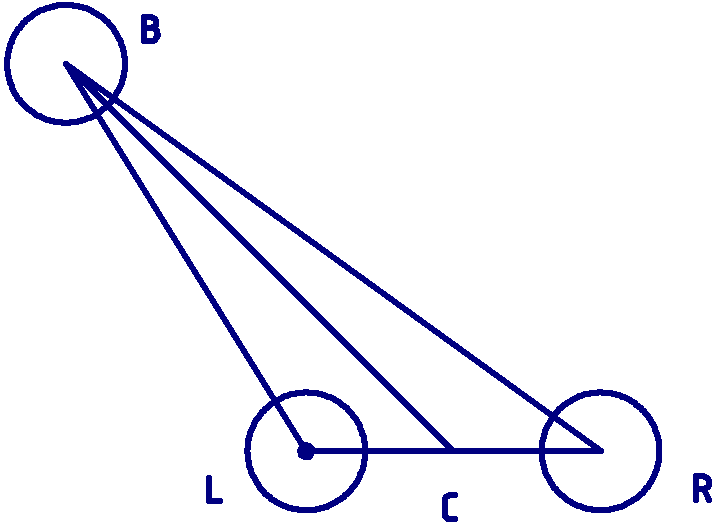
\includegraphics[width=0.5\textwidth]{images/PLANIMETRIA.png}
         \caption{\label{fig2}Planimetria}
    \end{figure}

    Conseguentemente il punto $C$ diventerà il centro della nostra coppia main. $CB$ quindi è la distanza tra il centro della coppia main e lo spot che vogliamo pannare.
    Ora è necessario effettuare tutti i calcoli trigonometrici per far si che L e R risultino due entità a parte. Questa operazione è il fulcro del nostro progetto, dato che ci permette di formalizzare, in seguito quella che è la vera differenza di fase, ampiezza e tempo tra il canale di sinistra e il canale di destra, in modo da effettuare un posizionamento nell'immagine stereofonica il più fedele possibile. Consideriamo di star comunque costruendo un modello matematico e non fisico: riusciamo quindi ad emulare solo parte del comportamento del nostro luogo fisico, tralasciando però, ad esempio, l'interazione della sorgente con l'ambiente. Le finalità del progetto quindi sono più chiare: non è ovviamente possibile simulare completamente un comportamento non deterministico in maniera deterministica.
    Ora quindi richiamiamo le funzioni già adoperate in precedenza per calcolarci $LB$ e $RB$ \\
    
    \begin{lstlisting}
//DISTANZA REALE TRA CIASCUN MIC DELLA COPPIA MAIN E LA SORGENTE
dstmicmain(cd,da,ab,dst,rad) = dstsource(cb,dst,rad)
with{
    cb = xyz2dst(cd,da,ab);
    dstsource(cb,dst,rad) = ts.lcarnot(cb,dst/2,rad);
};
    \end{lstlisting}
    
    In tal maniera, definiamo la funzione $dstmicmain$ che richiameremo 2 volte: una per calcolare $LB$ e l'altra per calcolare $RB$.
    Come ben noto, la sorgente $B$ avrà un angolo di incidenza differente su $L$ e su $R$. Quindi dobbiamo calcolarci anche queste misure adoperando, come in precedenza, il teorema di Carnot.
    \footnote{Ad esempio: consideriamo $CB = 40 cm$, $LR = 20cm$ (quindi $LC=10cm$) e l'angolo $\widehat{BCR} = 135°$ (così come avviene nella planimetria della Fig. 2). L'angolo d'incidenza su $L$ sarà uguale a $122.88$ e su $R$ sarà $180-36.46=143.54$. Contando che l'orecchio umano è capace di percepire una differenza di un grado frontale - cosa che ovviamente non avviene nel cono di confusione, anche queste piccole differenze aiutano a percepire meglio l'effetto del nostro panner}
    
    \begin{lstlisting}
//ANGOLO DI INCIDENZA DELLA SORGENTE SU UNA CAPSULA
radmicmain(cd,da,ab,dst,rad) = inc(dst,dstcap,cb)
with{
    cb = xyz2dst(cd,da,ab);
    dstcap = dstmicmain(cd,da,ab,dst,rad);
    
    inc(dst,dstcap,cb) = ts.acarnot(dst/2,dstcap,cb) : ts.rad2deg : (90-_) : ts.deg2rad;
};
    \end{lstlisting}

    La parte dove si fa la differenza $(90-_)$ è fondamentale in quanto, matematicamente, la figura polare cardioide, nella sua definizione, è orientata sull'asse x. Quindi è necessario correggere l'angolo in base a questo dato.\\
\subsection{Il ritardo tra i due microfoni main}
    La velocità del suono influisce sulle differenze di tempo, quindi è necessario costruire una funzione che, prese in input le distanze tra la sorgente e ciascuna capsula microfonica, calcoli un ritardo attraverso un valore di velocità arbitrario, che in questo caso sarà $321 m/s$

    \begin{lstlisting}
delaysig(sig,dst) = output(sig,delinsamples)
with {
    sspeed = 321;
    delinsamples = ((dst/100)/sspeed)*ma.SR : int;
    output(sig,delinsamples) = sig : de.delay(10000,delinsamples);
};
    \end{lstlisting}
    
\subsection{L'attenuazione}
    Altro dato importante è l'attenuazione del segnale in base alla distanza. Approssimativamente sappiamo che l'attenuazione è pari a 6 dB per ogni raddoppio della distanza. La nostra formula di attenuazione, ovviamente, è comunque approssimativa in quanto l'attenuazione non avviene linearmente per tutto lo spettro di frequenze della sorgente. Inoltre, la composizione dello spazio acustico e tutti i materiali influiscono molto sull'attenuazione. Poiché stiamo costruendo un modello matematico ideale, adoperiamo una formula di attenuazione che approssimi al meglio la resa sonora in un ambiente ideale. Nel nostro caso\\
    $$Att = \biggl({100 - 20*log_{10}(dst/0.1)\over100} \biggr)$$
\begin{lstlisting}
att(sig,dst) = output(sig,dst)
with{
    //Leq=Lrif-20*Log10(r/rrif)
    output(sig,dst) = sig * (100 - 20*log10(dst/0.1))/100;
};
\end{lstlisting}

\subsection{Il panning e la funzione main}
Definiamo l'ultima funzione panner che ci permette di simulare la figura polare cardioide e omnidirezionale. 
\begin{lstlisting}
panner(sig,pp,inc,dvg) = pan(sig,pp,inc,dvg)
with {
    pan(sig,pp,inc,dvg) = ppattern(sig,pp,inc,dvg); 
};
\end{lstlisting}

Come ultima cosa racchiudiamo tutte le funzioni precedentemente definite in un'unica funzione main "multipanner".

\begin{lstlisting}
multipanner(sig,cd,da,ab,dst,dvg,pp) = l(sig,pp,incL,dvg,dstL), r(sig,pp,incR,dvg,dstR)
with{
    //angolo dal centro
    radL = dst2arad(cd,da,ab);
    //a sinistra avremo l'angolo supplementare
    radR = radL : rad2deg : (_-180) : deg2rad;

    //calcolo angolo di incidenza su destra e sinistra
    incL = radmicmain(cd,da,ab,dst,radL);
    incR = radmicmain(cd,da,ab,dst,radR);

    //calcolo distanza effettiva sulla capsula di destra e quella di sinistra
    dstL = dstmicmain(cd,da,ab,dst,radL);
    dstR = dstmicmain(cd,da,ab,dst,radR);

    //calcolo finale ed applicazione del panning, dei delay e dell'attenuazione sia su L che su R.
    l(sig,pp,incL,dvg,dstL) = panner(sig,pp,incL,dvg) : delaysig(_,dstL) : att(_,dstL);
    r(sig,pp,incR,dvg,dstR) = panner(sig,pp,incR,-dvg) : delaysig(_,dstR) : att(_,dstR);
};

process = multipanner(_,cd, da, ab, dst, dvg, pp);
\end{lstlisting}
    \begin{figure}[H]
        \centering
        \includegraphics[width=0.5\textwidth]{images/225.png}
         \caption{\label{fig10}Posizione del segnale a 225°}
    \end{figure}

    Se immaginiamo, invece, di avere il segnale esattamente a 90° in una figura a 8: \\
    mid=((1-1*segnale)+(1*segnale*cos(90°)) = 0 - cioè annullamento completo del mid side=segnale*sin(90°) = L e R tra loro in controfase.

\section{Differenze con un panner tradizionale}
    \subsection{Cenni sulla stereofonia}
    
    Un panner tradizionale LR - meglio detto balance, ha come unica variabile la differenza d'ampiezza tra sinistra a destra. È facile intuire che questo potrebbe essere molto limitante in quanto non ci da una informazione stereofonica. La stessa parola "stereofonica" deriva dal greco antico, in particolare dall'unione delle parole "sterèos" (in italiano "stabile", "solido", ma anche "spaziale", "tridimensionale") e "phonè" (in italiano "suono"). La percezione della tridimensionalità del suono nello spazio per l'uoomo è data da tre parametri fondamentali, ovverosia ITD (Interaural Time Difference), ILD (Interaural Level Difference), DDF (Direction Dependent Filter). La prima riguarda la differenza di tempo che intercorre tra l'orecchio sinistro e quello destro che, la seconda riguarda l'ampiezza e la terza riguarda l'alterazione del contenuto spettrale percepito da Sx e Dx in base alla posizione della sorgente.
    Poiché l'obiettivo è quello di fornire uno strumento che adoperi sul panorama stereo, è importante tener conto non solo della fisicità della coppia stereo, ma anche di tutti i parametri prettamente percettivi della stereofonia. Infatti il progetto non solo nasce come strumento da applicare per la costruzione di un panorama stereo verosimile ad una coppia ORTF, ma anche come strumento creativo adoperabile a fini tecnici e/o compositivi.

    \subsection{Le variabili}
    Prendendo in considerazione quanto detto su ITD, ILD e DDF, comprendiamo che non è sufficiente descrivere un comportamento stereofonico basandosi solo su unico parametro come avviene nel panner tradizionale. Difatti nel nostro caso abbiamo provveduto non solo a differenziare l'ampiezza, ma anche a fornire una differenza di tempo tra L e R e una spettrale. Così facendo ampliamo le possibilità di utilizzo del progetto che, come già accennato, può anche essere utilizzato a fini creativi.

\section{Vantaggi, svantaggi e future migliorie}

\subsection{$x, y, \Delta z$}
    Lo strumento nasce per avere una scientificità nella posizione del panorama stereo. Di conseguenza sarebbe opportuno approcciare ad uno strumento "scientifico" - se non per scopi creativi - con un metodo altrettanto "scientifico".
    Durante la prima applicazione del panner, non disponendo di misure precise di distanze $x, y, \Delta z$ , i risultati sono stati buoni, ma comunque con un margine di errore - nel nostro caso - trascurabile.
    Fatto sta che per ricavare tali misure è stato necessario non solo fare i rilievi delle distanze sul posto, ma anche fare un disegno tecnico della realtà di riferimento. Conseguentemente, in alcune situazioni potrebbe risultare scomodo utilizzare questo strumento se non si hanno degli adeguati strumenti di misurazione o delle adeguate competenze per fare un disegno tecnico. All'atto pratico il calcolo di  $x, y, \delta z$, però, è l'unico scoglio da superare nell'utilizzo del Multipanner.

\subsection{La velocità del suono}
    Nel caso dell'utilizzo dei panner in un multitraccia di un'orchestra, uno dei vantaggi di avere dei delay su L e su R è quello di effettuare automaticamente l'allineamento di tutte le take degli spot verso la coppia main, evitando di effettuare il Ciak. Però c'è da considerare un problema: è abbastanza complesso rilevare la velocità del suono. Difatti noi nella definizione del multipanner, abbiamo utilizzato un valore convenzionale, nonché $321 m/s$. Per offrire una maggiore scientificità allo strumento, sarebbe opportuno anche inserire una funzione di allineamento che rilevi automaticamente la velocità del suono nell'ambiente considerato - anche se non avremo mai una misura precisa al millesimo.
    
\subsection{Comb Filtering}
    Le differenze di tempo tra L e R fanno si che, nel caso della loro somma, ci siano fenomeni di comb filtering. Sarebbe quindi opportuno aggirare almeno parzialmente il problema lavorando a frequenze di campionamento più alte. Per evitare completamente il comb filtering, in una seconda versione, sarà integrata una parte di filtri allpass che correggono le cancellazioni di fase su tutto lo spettro.

\end{document}